\documentclass[a4]{article}
\pagestyle{myheadings}

%%%%%%%%%%%%%%%%%%%
% Packages/Macros %
%%%%%%%%%%%%%%%%%%%
\usepackage{mathrsfs}


\usepackage{fancyhdr}
\pagestyle{fancy}
\lhead{}
\chead{}
\rhead{}
\lfoot{}
\cfoot{} 
\rfoot{\normalsize\thepage}
\renewcommand{\headrulewidth}{0pt}
\renewcommand{\footrulewidth}{0pt}
\newcommand{\RomanNumeralCaps}[1]
    {\MakeUppercase{\romannumeral #1}}

\usepackage{amssymb,latexsym}  % Standard packages
\usepackage[utf8]{inputenc}
\usepackage[russian]{babel}
\usepackage{MnSymbol}
\usepackage{mathrsfs}
\usepackage{amsmath,amsthm}
\usepackage{indentfirst}
\usepackage{graphicx}%,vmargin}
\usepackage{graphicx}
\graphicspath{{pictures/}} 
\usepackage{verbatim}
\usepackage{color}
\usepackage{color,colortbl}
\usepackage[nottoc,numbib]{tocbibind}
\usepackage{float}
\usepackage{multirow}
\usepackage{hhline}

\usepackage{listings}
\definecolor{codegreen}{rgb}{0,0.6,0}
\definecolor{codegray}{rgb}{1,1,1}
\definecolor{codepurple}{rgb}{0.58,0,0.82}
\definecolor{backcolour}{rgb}{0.95,0.95,0.92}
 
\lstdefinestyle{mystyle}{
    backgroundcolor=\color{backcolour},   
    commentstyle=\color{codegreen},
    keywordstyle=\color{magenta},
    numberstyle=\tiny\color{codegray},
    stringstyle=\color{codepurple},
    basicstyle=\footnotesize,
    breakatwhitespace=false,         
    breaklines=true,                 
    captionpos=b,                    
    keepspaces=true,                 
    numbers=left,                    
    numbersep=5pt,                  
    showspaces=false,                
    showstringspaces=false,
    showtabs=false,                  
    tabsize=2
}
 
\lstset{style=mystyle}

\usepackage{url}
\urldef\myurl\url{foo%.com}
\def\UrlBreaks{\do\/\do-}
\usepackage{breakurl}
\Urlmuskip=0mu plus 1mu



\DeclareGraphicsExtensions{.pdf,.png,.jpg}% -- настройка картинок

\usepackage{epigraph} %%% to make inspirational quotes.
\usepackage[all]{xy} %for XyPic'a
\usepackage{color} 
\usepackage{amscd} %для коммутативных диграмм
%\usepackage[colorlinks,urlcolor=red]{hyperref}

%\renewcommand{\baselinestretch}{1.5}
%\sloppy
%\usepackage{listings}
%\lstset{numbers=left}
%\setmarginsrb{2cm}{1.5cm}{1cm}{1.5cm}{0pt}{0mm}{0pt}{13mm}


\newtheorem{Lemma}{Лемма}[section]
\newtheorem{Proposition}{Предложение}[section]
\newtheorem{Theorem}{Теорема}[section]
\newtheorem{Corollary}{Следствие}[section]
\newtheorem{Remark}{Замечание}[section]
\newtheorem{Definition}{Определение}[section]
\newtheorem{Designations}{Обозначение}[section]




%%%%%%%%%%%%%%%%%%%%%%% 
%Подготовка оглавления% 
%%%%%%%%%%%%%%%%%%%%%%% 
\usepackage[titles]{tocloft}
\renewcommand{\cftdotsep}{2} %частота точек
\renewcommand\cftsecleader{\cftdotfill{\cftdotsep}}
\renewcommand{\cfttoctitlefont}{\hspace{0.38\textwidth} \LARGE\bfseries} 
\renewcommand{\cftsecaftersnum}{.}
\renewcommand{\cftsubsecaftersnum}{.}
\renewcommand{\cftbeforetoctitleskip}{-1em} 
\renewcommand{\cftaftertoctitle}{\mbox{}\hfill \\ \mbox{}\hfill{\footnotesize Стр.}\vspace{-0.5em}} 
%\renewcommand{\cftchapfont}{\normalsize\bfseries \MakeUppercase{\chaptername} } 
%\renewcommand{\cftsecfont}{\hspace{1pt}} 
\renewcommand{\cftsubsecfont}{\hspace{1pt}} 
%\renewcommand{\cftbeforechapskip}{1em} 
\renewcommand{\cftparskip}{3mm} %определяет величину отступа в оглавлении
\setcounter{tocdepth}{5} 
\renewcommand{\listoffigures}{\begingroup %добавляем номер в список иллюстраций
\tocsection
\tocfile{\listfigurename}{lof}
\endgroup}
\renewcommand{\listoftables}{\begingroup %добавляем номер в список иллюстраций
\tocsection
\tocfile{\listtablename}{lot}
\endgroup}


%\renewcommand{\thelikesection}{(\roman{likesection})}
%%%%%%%%%%%
% Margins %
%%%%%%%%%%%
\addtolength{\textwidth}{0.7in}
\textheight=630pt
\addtolength{\evensidemargin}{-0.4in}
\addtolength{\oddsidemargin}{-0.4in}
\addtolength{\topmargin}{-0.4in}

%%%%%%%%%%%%%%%%%%%%%%%%%%%%%%%%%%%
%%%%%%Переопределение chapter%%%%%% 
%%%%%%%%%%%%%%%%%%%%%%%%%%%%%%%%%%%
\newcommand{\empline}{\mbox{}\newline} 
\newcommand{\likechapterheading}[1]{ 
\begin{center} 
\textbf{\MakeUppercase{#1}} 
\end{center} 
\empline} 

%%%%%%%Запиливание переопределённого chapter в оглавление%%%%%% 
\makeatletter 
\renewcommand{\@dotsep}{2} 
\newcommand{\l@likechapter}[2]{{\bfseries\@dottedtocline{0}{0pt}{0pt}{#1}{#2}}} 
\makeatother 
\newcommand{\likechapter}[1]{ 
\likechapterheading{#1} 
\addcontentsline{toc}{likechapter}{\MakeUppercase{#1}}} 




\usepackage{xcolor}
\usepackage{hyperref}
\definecolor{linkcolor}{HTML}{000000} % цвет ссылок
\definecolor{urlcolor}{HTML}{3643FF} % цвет гиперссылок
 
\hypersetup{pdfstartview=FitH,  linkcolor=linkcolor,urlcolor=urlcolor, colorlinks=true}

%%%%%%%%%%%%
% Document %
%%%%%%%%%%%%

%%%%%%%%%%%%%%%%%%%%%%%%%%%%%
%%%%%%главы -- section*%%%%%%
%%%%section -- subsection%%%%
%subsection -- subsubsection%
%%%%%%%%%%%%%%%%%%%%%%%%%%%%%
\def \newstr {\medskip \par \noindent} 



\begin{document}
\newcolumntype{g}{>{\columncolor{codegray}}c}



\def\contentsname{\LARGE{Содержание}}
\thispagestyle{empty}
	\begin{center} 
	\vspace{2cm} 
	{\Large \sc Санкт-Петербургский Политехнический Университет}\\
	\vspace{2mm}
	{\Large\sc им. Петра Великого}\\
	\vspace{1cm}
	{\large \sc Институт прикладной математики и механики\\ 
		\vspace{0.5mm}
		\textsc{}}\\ 
	\vspace{0.5mm}
	{\large\sc Кафедра $"$Прикладная математика$"$}\\
	\vspace{15mm}
	
	
	{\sc \textbf{Отчёт\\
			Лабораторная работа № 5\\
			по дисциплине\\
			"Математическая статистика"}
		\vspace{6mm}
		
	}
	\vspace*{2mm}
	
	
	\begin{flushleft}
		\vspace{4cm}
		\sc Выполнил студент:\\
		\sc Мальцов Дмитрий Дмитриевич\\
		\sc группа: 3630102/70401\\
		\vspace{1cm}
		\sc Проверил:\\
		\sc к.ф-м.н., доцент\\
		\sc Баженов Александр Николаевич
		\vspace{20mm}
	\end{flushleft}
\end{center} 
\begin{center}
	\vfill {\large\textsc{Санкт-Петербург}}\\ 
	2020 год
\end{center}

%%%%%%%%%%%%%%%%%%%%%%%%%%%%%%%%%%%%%%%%%%%%%%%%%%%%%%%%%%%%%%%%%%%%%%%%%%%%%%%%%%%%%%%%%%%%%%
%\ \\[4cm]

%\rm
%%%%%%%%%%%%%%%%%%%%%%%%%%%%%%%%%%%%%%%%%%%%%%%%%%%%%%%%%%%%%%%%%%%%%%%%%%%%%%%%%%%%%%%%%%%%%%
\newpage
\pagestyle{plain}

%\begin{center}
%\begin{abstract} 

%\end{abstract}

%\end{center}

\newpage
\tableofcontents{}
\newpage
\listoffigures{}
\listoftables{}
\newpage

\section{Постановка задачи}

Сгенерировать двумерные выборки размерами $20, 60, 100$ для двумерного нормального распределения $ N(x,y,0,0,1,1,\rho) $.
\par Коэффициент корреляции $\rho$ взять равным $0, 0.5, 0.9$.
\par Каждая выборка генерируется 1000 раз и для неё вычисляются: среднее значение, среднее значение квадрата и дисперсия коэффициентов корреляции Пирсона, Спирмена и квадрантного коэффициента корреляции.
Повторить все вычисления для смеси нормальных распределений: 
\begin{equation}
    f(x,y) = 0.9N(x,y,0,0,1,1,0.9)+0.1N(x,y,0,0,10,10,-0.9)
\end{equation}
Изобразить сгенерированные точки на плоскости и нарисовать эллипс равновероятности.


\section{Теория}

\begin{enumerate}
    \item Двумерное нормально распределение:
        \begin{multline}
        N(x,y,\bar{x},\bar{y},\sigma_{x},\sigma_{y},\rho)=\frac{1}{2\pi\sigma_{x}\sigma_{y}\sqrt{1-\rho^{2}}}\times\\
        \times exp(-\frac{1}{2(1-\rho^{2})}[\frac{(x-\bar{x})^{2}}{\sigma_{x}^{2}}-2\rho\frac{(x-\bar{x})(y-\bar{y})}{\sigma_{x}\sigma_{y}}+\frac{(y-\bar{y})^{2}}{\sigma_{y}^{2}}])
        \end{multline}
    
    \item Коэффициент корреляции Пирсона:
        \begin{equation}
        r=\frac{\frac{1}{n}\sum(x_{i}-\bar{x})(y_{i}-\bar{y})}{\sqrt{\frac{1}{n}\sum(x_{i}-\bar{x})^{2}\frac{1}{n}\sum(y_{i}-\bar{y})^{2}}}
        \end{equation}
        
        \item Квадрантный коэффициент корреляции:
        \begin{equation}
        r_{Q} = \frac{(n_{1} + n_{3}) - (n_{2} + n_{4})}{n}
        \end{equation}
        где $ n_{1},n_{2},n_{3},n_{4} $ -- количества точек с координатами $ (x_{i},y_{i}) $, попавшими соответственно в \RomanNumeralCaps{1},\RomanNumeralCaps{2},\RomanNumeralCaps{3} и \RomanNumeralCaps{4} квадранты декартовой системы с осями $x^{'}=x-med x, y^{'}=y-med y  $ и с центром в точке с координатами$ (med x, med y) $
    \item Коэффициент корреляции Спирмана:
        \begin{equation}
        r_{S}=\frac{\frac{1}{n}\sum(u_{i}-\bar{u})(v_{i}-\bar{v})}{\sqrt{\frac{1}{n}\sum(u_{i}-\bar{u})^{2}\frac{1}{n}\sum(v_{i}-\bar{v})^{2}}}
        \end{equation}
        где $ u $ и $ v $ -- ранги, соотвествующие значениям переменной $X$ и $ Y $ соответственно.
        
\end{enumerate}

\section{Реализация}
Работы была выполнена на языке $Python 3.8.2$
Для генерации выборок использовался модуль модуль $stats$ библиотеки $scipy$.
Для построения графиков использовалась библиотека matplotlib.

\section{Результаты}

\begin{table}[H]
	\caption{Двумерное нормальное распределение, $n=20$}
	\label{tab:my_label3}
	\begin{center}
		\vspace{5mm}
		\begin{tabular}{|c|c|c|c|}
			\hline
			$ \rho=0 $ & Pearson & Spearman & Quad\\
			\hline
			$ E(z) $ & $ 0.009 $ & $ 0.001 $ & $ 0.004 $\\
			\hline
			$ E(z^{2}) $ & $ 0.05 $ & $ 0.05 $ & $ 0.05 $\\
			\hline
			$ D(z) $  & $ 0.05 $ & $ 0.05 $ & $ 0.05 $\\
			\hline
			$ \rho=0.5 $ & Pearson & Spearman & Quad\\
			\hline
			$ E(z) $ & $ 0.49 $ & $ 0.46 $ & $ 0.32 $\\
			\hline
			$ E(z^{2}) $ & $ 0.27 $ & $ 0.25 $ & $ 0.15 $\\
			\hline
			$ D(z) $  & $ 0.03 $ & $ 0.03 $ & $ 0.05 $ \\
			\hline
			$ \rho=0.9 $ & Pearson & Spearman & Quad\\
			\hline
			$ E(z) $ & $ 0.893 $ & $ 0.865 $ & $ 0.69 $\\
			\hline
			$ E(z^{2}) $ & $ 0.801 $ & $ 0.754 $ & $ 0.5 $\\
			\hline
			$ D(z) $  & $ 0.003 $ & $ 0.05 $ & $ 0.03 $ \\
			\hline
		\end{tabular}
	\end{center}
\end{table}

\begin{table}[H]
	\caption{Двумерное нормальное распределение, $n=60$}
	\label{tab:my_label3}
	\begin{center}
		\vspace{5mm}
		\begin{tabular}{|c|c|c|c|}
			\hline
			$ \rho=0 $ & Pearson & Spearman & Quad\\
			\hline
			$ E(z) $ & $ -0.003 $ & $ -0.004 $ & $ -0.0004 $\\
			\hline
			$ E(z^{2}) $ & $ 0.02 $ & $ 0.2 $ & $ 0.02 $\\
			\hline
			$ D(z) $  & $ 0.02 $ & $ 0.02 $ & $ 0.02 $\\
			\hline
			$ \rho=0.5 $ & Pearson & Spearman & Quad\\
			\hline
			$ E(z) $ & $ 0.497 $ & $ 0.47 $ & $ 0.33 $\\
			\hline
			$ E(z^{2}) $ & $ 0.257 $ & $ 0.24 $ & $ 0.13 $\\
			\hline
			$ D(z) $  & $ 0.009 $ & $ 0.01 $ & $ 0.02 $ \\
			\hline
			$ \rho=0.9 $ & Pearson & Spearman & Quad\\
			\hline
			$ E(z) $ & $ 0.8984 $ & $ 0.883 $ & $ 0.706 $\\
			\hline
			$ E(z^{2}) $ & $ 0.8078 $ & $ 0.782 $ & $ 0.508 $\\
			\hline
			$ D(z) $  & $ 0.0007 $ & $ 0.001 $ & $ 0.009 $ \\
			\hline
		\end{tabular}
	\end{center}
\end{table}

\begin{table}[H]
	\caption{Двумерное нормальное распределение, $n=100$}
	\label{tab:my_label3}
	\begin{center}
		\vspace{5mm}
		\begin{tabular}{|c|c|c|c|}
			\hline
			$ \rho=0 $ & Pearson & Spearman & Quad\\
			\hline
			$ E(z) $ & $ -0.004 $ & $ -0.004 $ & $ -0.001 $\\
			\hline
			$ E(z^{2}) $ & $ 0.01 $ & $ 0.01 $ & $ 0.01 $\\
			\hline
			$ D(z) $  & $ 0.01 $ & $ 0.01 $ & $ 0.01 $\\
			\hline
			$ \rho=0.5 $ & Pearson & Spearman & Quad\\
			\hline
			$ E(z) $ & $ 0.499 $ & $ 0.481 $ & $ 0.329 $\\
			\hline
			$ E(z^{2}) $ & $ 0.254 $ & $ 0.237 $ & $ 0.118 $\\
			\hline
			$ D(z) $  & $ 0.005 $ & $ 0.006 $ & $ 0.009 $ \\
			\hline
			$ \rho=0.9 $ & Pearson & Spearman & Quad\\
			\hline       
			$ E(z) $ & $ 0.8981 $ & $ 0.8841 $ & $ 0.708 $\\
			\hline
			$ E(z^{2}) $ & $ 0.8071 $ & $ 0.7823 $ & $ 0.506 $\\
			\hline
			$ D(z) $  & $ 0.0004 $ & $ 0.0007 $ & $ 0.004 $ \\
			\hline
		\end{tabular}
	\end{center}
\end{table}

\begin{table}[H]
	\caption{Смесь нормальных распределений}
	\label{tab:my_label3}
	\begin{center}
		\vspace{5mm}
		\begin{tabular}{|c|c|c|c|}
			\hline
			$ n=20 $ & Pearson & Spearman & Quad\\
			\hline
			$ E(z) $ & $ -0.09 $ & $ -0.09 $ & $ -0.06 $\\
			\hline
			$ E(z^{2}) $ & $ 0.05 $ & $ 0.06 $ & $ 0.06 $\\
			\hline
			$ D(z) $  & $ 0.05 $ & $ 0.05 $ & $ 0.05 $\\
			\hline
			$ n=60 $ & Pearson & Spearman & Quad\\
			\hline
			$ E(z) $ & $ -0.09 $ & $ -0.004 $ & $ -0.06 $\\
			\hline
			$ E(z^{2}) $ & $ 0.03 $ & $ 0.02 $ & $ 0.02 $\\
			\hline
			$ D(z) $  & $ 0.02 $ & $ 0.02 $ & $ 0.02 $ \\
			\hline
			$ n=100 $ & Pearson & Spearman & Quad\\
			\hline       
			$ E(z) $ & $ -0.094 $ & $ -0.079 $ & $ -0.06 $\\
			\hline
			$ E(z^{2}) $ & $ 0.018 $ & $ 0.016 $ & $ 0.01 $\\
			\hline
			$ D(z) $  & $ 0.009 $ & $ 0.009 $ & $ 0.01 $ \\
			\hline
		\end{tabular}
	\end{center}
\end{table}

%\vspace{-2cm}
\begin{figure}[H]
    \centering
    \caption{Графики двумерного нормального распределения и смеси для размера выборки $ n =20 $ }
    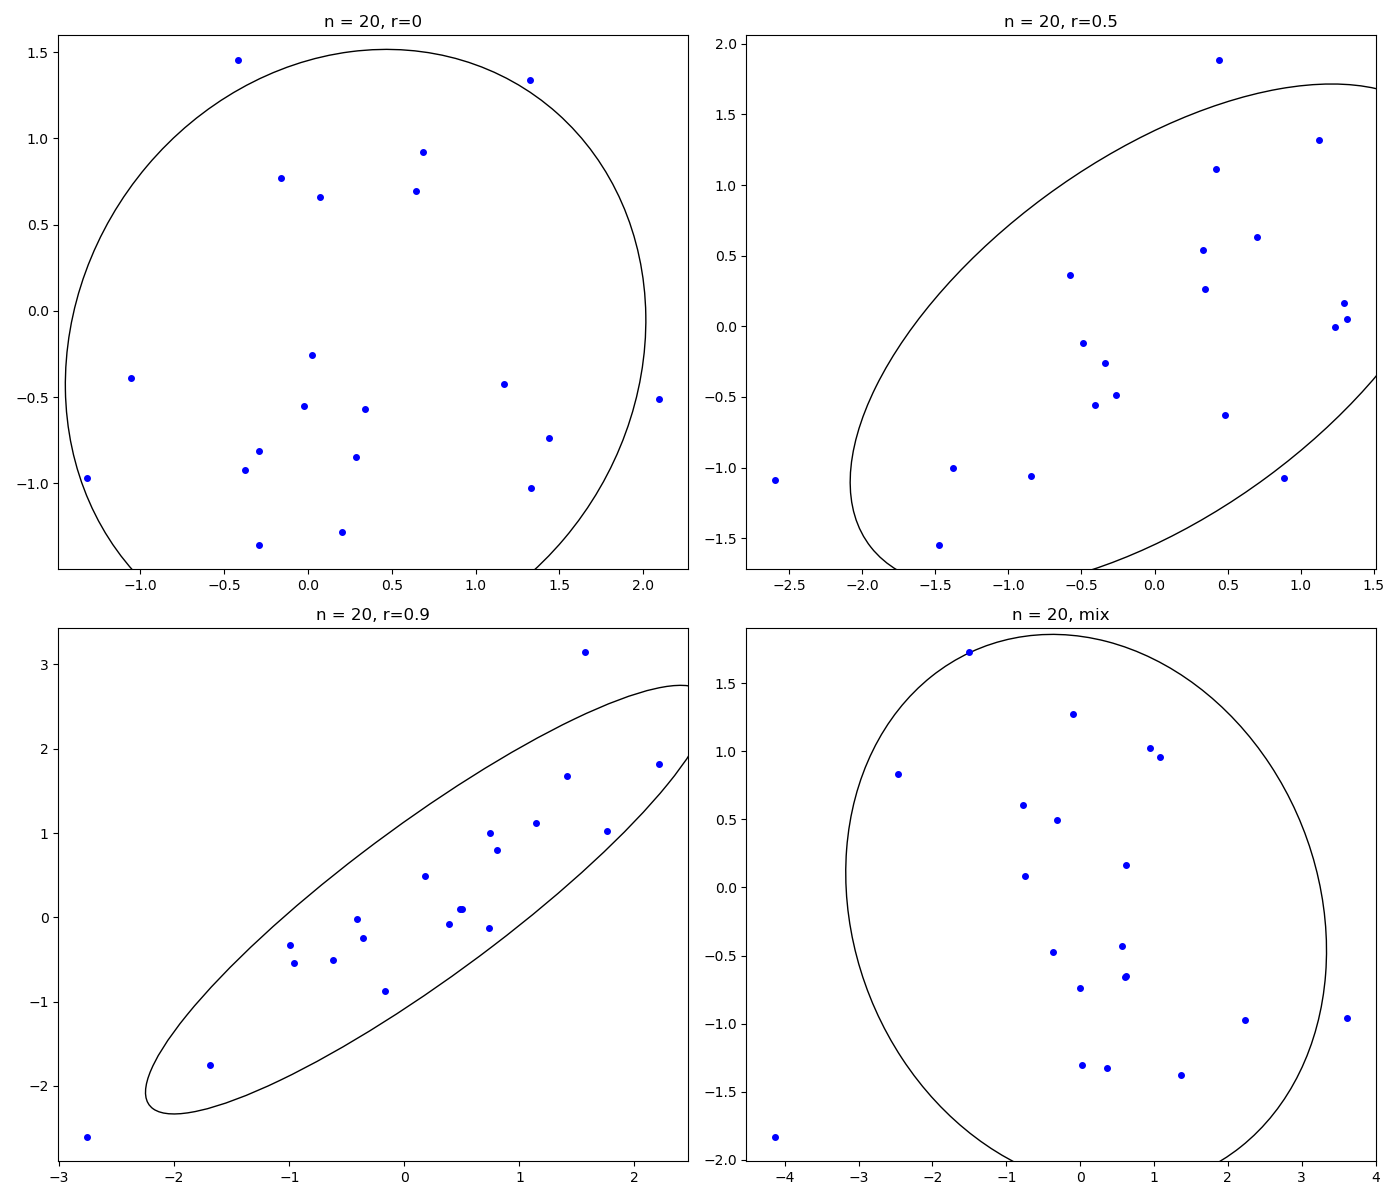
\includegraphics[scale = 0.5]{ellipse_n=20.png} 
    \label{fig:dis_norm_gis0}
\end{figure}

\vspace{-10cm}
\begin{figure}[H]
    \centering
    \caption{Графики двумерного нормального распределения и смеси для размера выборки $ n =60 $ }
    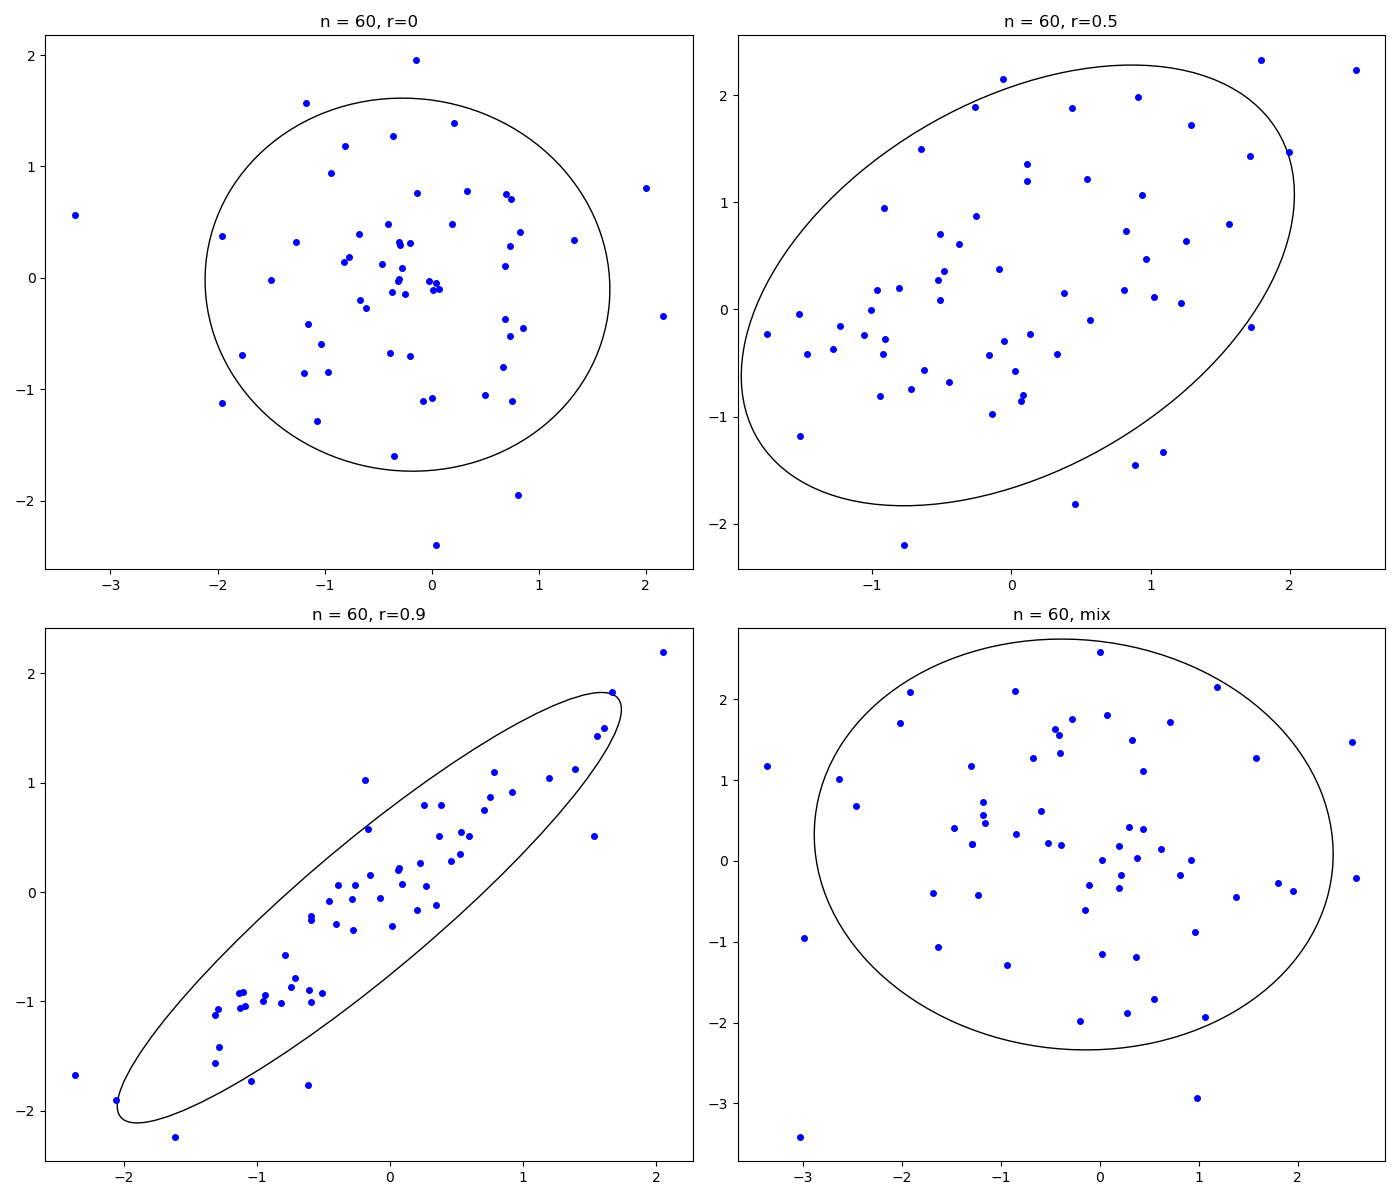
\includegraphics[scale = 0.5]{ellipse_n=60.png}
    \label{fig:dis_norm_gis1}
\end{figure}

\vspace{-1cm}
\begin{figure}[H]
    \centering
    \caption{Графики двумерного нормального распределения и смеси для размера выборки $ n =100 $ }
    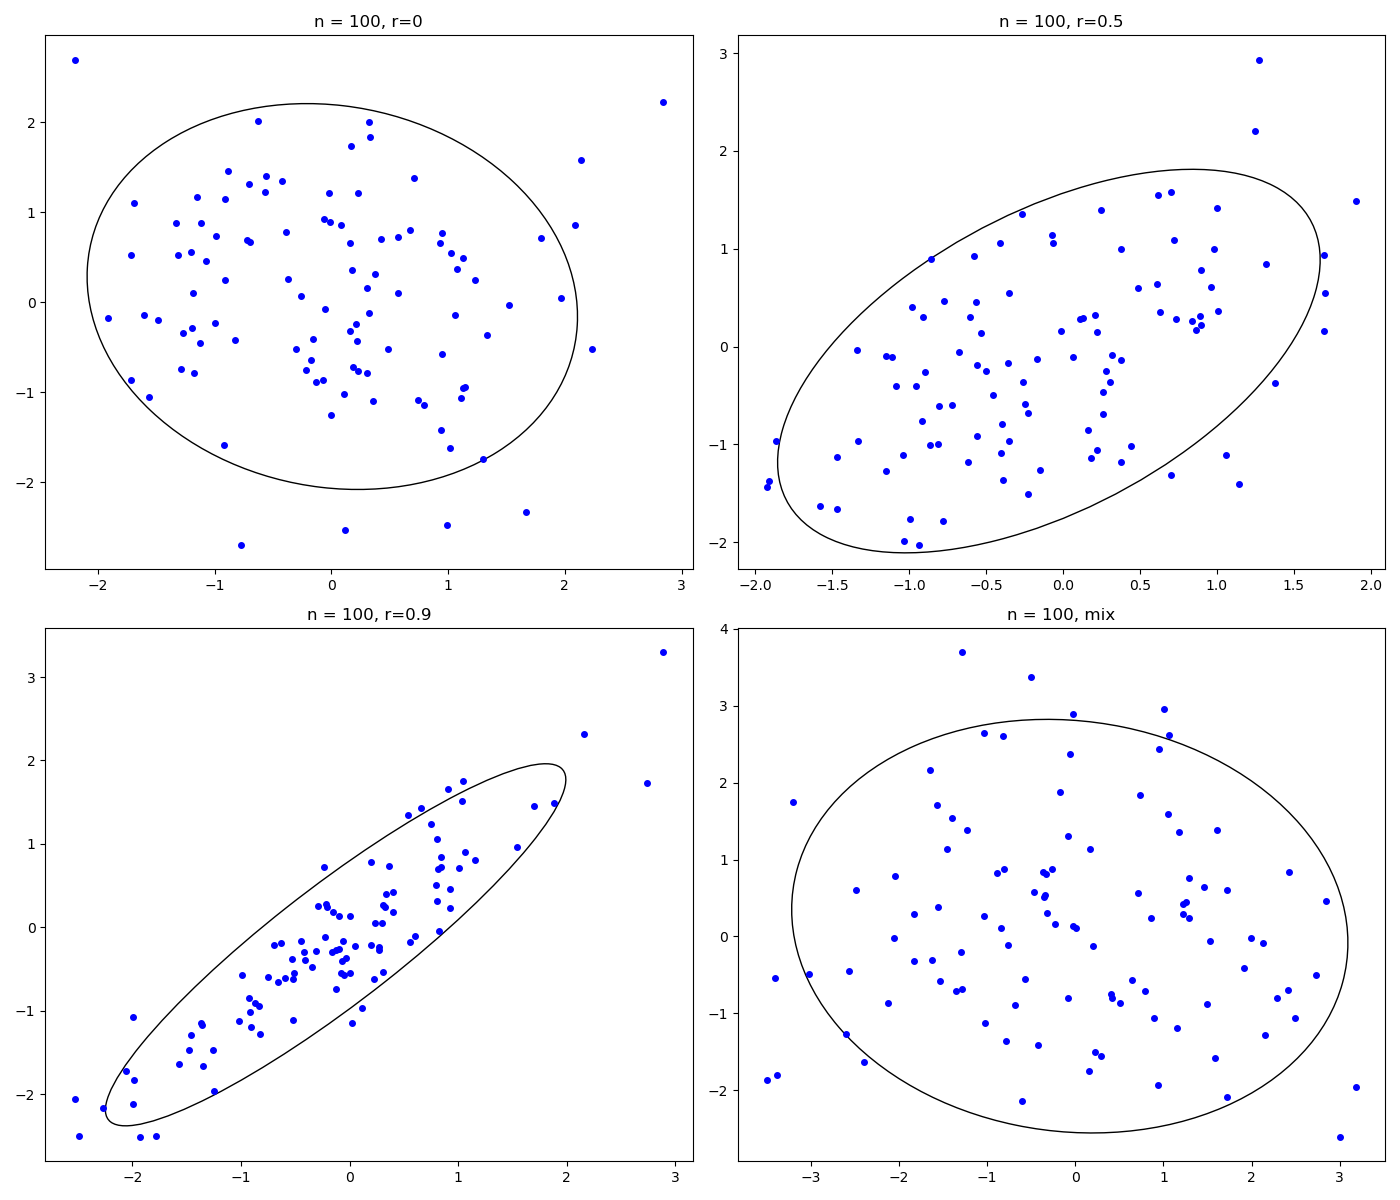
\includegraphics[scale = 0.5]{ellipse_n=100.png} 
    \label{fig:dis_norm_gis2}
\end{figure}

\begin{figure}[H]
	\centering
	\caption{Графики эллипса рассеивания для двумерного нормального распределения для $ 2 $ точек }
	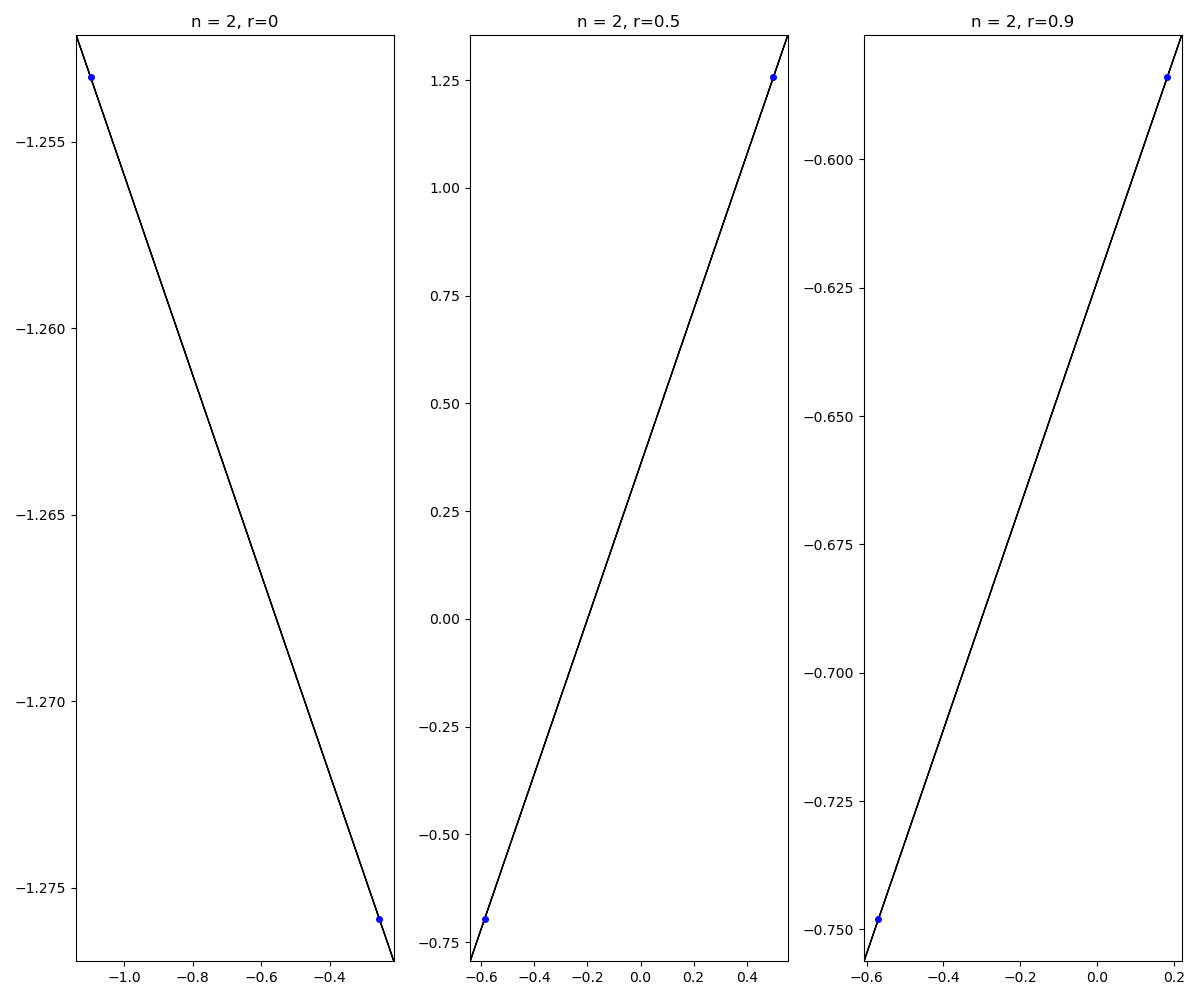
\includegraphics[scale = 0.5]{ellipse_n=2.png} 
	\label{fig:dis_norm_gis2}
\end{figure}

\begin{figure}[H]
	\centering
	\caption{Графики эллипса рассеивания для двумерного нормального распределения для $ 3 $ точек }
	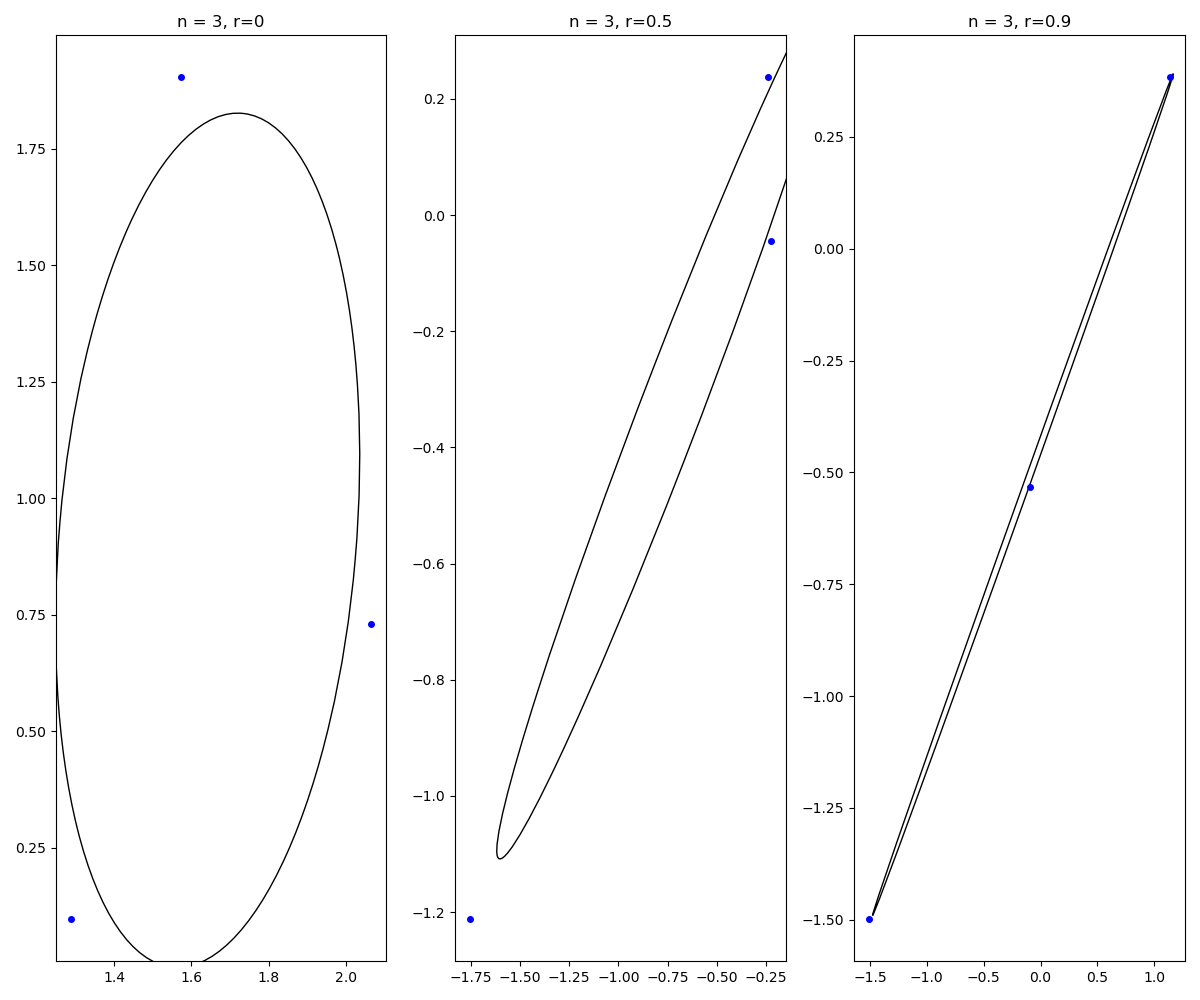
\includegraphics[scale = 0.5]{ellipse_n=3.png} 
	\label{fig:dis_norm_gis2}
\end{figure}

\section{Выводы}
По графикам, видно, что, при увеличении объёма выборки, подсчитанные коэффициенты корреляции стремятся к теоретическим.

Ближе всего к теоретическому коэффициенту корреляции находится коэффициент Пирсона.

По графикам также видно, что при уменьшении корреляции эллипс равновероятности стремится к окружности, а при увеличении растягивается, стремясь к прямой.

Из графиков наглядно видно, что для построения эллипса рассеивания необходимое минимальное число событий в выборке -- 3 события, так как 2 точки (2 события) вырождаются в прямую линию ( для 2 точек мы всегда можем перейти в систему координат, где у одной из компонент вектора (x,y) будет 0 мат. ожидание и 0 дисперсия, то есть переходим в одномерный случай).

\section{Литература}

\href{https://physics.susu.ru/vorontsov/language/numpy.html}{Модуль numpy}\\

\href{https://matplotlib.org/}{Модуль matplotlib}\\

\href{https://www.scipy.org/}{Модуль scipy}\\


\section{Приложения}

\href{https://github.com/dmitry-maltsov/PolyMatStat/blob/master/5/lab5.py}{Код лабораторной}


\end{document}
